% Replace 'text' below with your text.  Use \citep{Author2016} to add a
% parenthetical citation; use \citet{Author2016} to get a textual cite like
% this: Author (2016).  FS will add the code to insert figures.

\section{Use Consistent Measures}
Properly using measurements is the next critical step in empirical analysis after data collection. It is the crucial stage transforming abstract theoretical concepts to operable data for later empirical tests, which directly determines the internal validity of the study. According to \cite{Hunter2001} and \cite{Hamermesh2007}, internal validity can be divided into two types, statistical replication and scientific replication. Besides the latter about the external validity, the former  particularly relates to the choice and manipulation of measurements, which refers to that ``[w]hen a researcher uses a different sample from the same population to evaluate the same theoretical implication as in the previous study with equivalent construct validity...'' \cite[258]{Morton2010}. Stated differently, to validate a study, the researcher should conduct tests on theoretically equivalent measures all the way. This criterion should be taken into account not only in the robustness tests section of a study but also when the main variables are originally measured. 

To achieve this criterion, a researcher should consider about three ``consistencies'': first, \textit{data source consistency}. All the steps in designs and implements of data collection may lead to substantively different results. To minimize measurement error or at least keep it in a coherent way so as to eliminate later, we suggest researchers to use consistent data source, in which the data are collected and coded in a consistent manner. This becomes an issue especially if the researchers is considering create measures from multiple available data sources . In such case, except for validating the measure in general fit the theory they intend to test, the researchers should carefully review the data collection and coding process to ensure that the data collected in each data set reflect the same concept. For example, in a cross-survey study, one should select data produced by the similar questions for each variable. 

Taking the aforementioned case, \cite{Newman2015}, for measuring the dependent variable, they used 2005, 2006, 2007, and 2009 surveys on the US citizens conducted by Pew Research Center. For 2005 and 2006, they used responses from exactly the same question. This strategy guarantees data coming from the same organizers, for the same question in same area, and therefore reduces the risk to violate the inconsistency in the data. Researchers should also be aware that any above ``sames'' singly is not a sufficient condition for measurement consistency. In the previous case, for data from 2007 to 2009, researcher still chose the data from the same organizer and in the same area, but with different questions and coding methods. As shown in the later test, the measurement no longer captured the same concept. Another example is from Asia Barometer. \cite{Chu2010} found that responses on the same question about the attitude towards democracy did not capture the public attitude to democracy in the theoretical sense, but reflected different understandings of this concept in the given political environment \cite[see, also, ][]{Lu2014a}.

Unfortunately, in reality, we may not always enable to keep exactly data source consistency because of the limitation in data availability. In such case, researchers should not let this issue to stop them to sufficiently use all available data (as we suggested in \cref{S:data}), while they have to be very careful to combine and manipulate data. Doing them inappropriately may distort data and introduce serious biases into the analysis. To minimize this risk, researchers are ought to consider at least two issues: \textit{structural consistency} and \textit{method consistency}. The structural consistency refers to the consistency in the data coding format. Different format may capture different aspects of a concept which may not be comparable. A famous case of it is the measurement debate on challenges of \cite{Przeworski2000} on the classic developmentalist argument about democratization by \cite{Lipset1960}. The former went against the conclusion of the latter arguing that economic development is not a necessary condition for democratization. Nevertheless, in the empirical tests, Przeworski et al. used a binary variable for degree of democracy and only used income to measure development. This led the concern about whether their test truly reject Lipset's theory or just capture a different aspect of the democratization process \cite[not very sure if this citation is adequate][]{Bernhagen2009}. Another example is from the previous case of \cite{Newman2015}.

For 2005 and 2006, they used public attitudes towards two statements ``Most people who want to get ahead can make it if they're willing to work hard'' or ``Hard work and determination are no guarantee of success for most people.'' If the respondents agree with the first one, they got 1; if they agree with the second, then 0. The result measure is an aggregated binary variable based on two binary survey questions. For 2007, they chose the questions asking the attitudes towards the two statements separately. For each statement, there is a 4-scale categorical recorded from ``completely agreed'' to ``completely disagreed.'' When respondents answered completely or mostly agree to \textit{both} statements, they got 1, otherwise, 0. For the 2009 data, Newman et al. only used the records for the second attitude, even if the question about the first attitude was also asked in the survey as in 2007. For this year, then, respondents only needed to answer ``completely agreed'' or ``mostly agreed'' for the second statement to get 1 in Newman et al. measure of the dependent variable. 

The authors in this case not only used data with inconsistent format, which we admitted being unavoidable only when data with the same structure is unavailable, but also had a method inconsistency issue. They used three different methods to convert survey records to binary. This could make the measure very tricky, since the variance in the measure could also be caused or changed due to the applications of multiple methods. 

Our test confirms this concern. We apply each of the three measurements Newman et al. used on structurally consistent data from 1999 to 2012. \cref{F:three_measures} presents the results. The plot clearly illustrates how different the result from the three methods. Measure 2 is systematically lower than Measure 1 and 3; even if for 1 and 3, they follow very different patterns, except for a couple of dyadic crosses.\footnote{We even extend the testing to all the available datasets to 1987 - 2003, and account for the uncertainty in the samples. The result shown in \cref{A:dotwhisker} manifests that except for a couple of overlaps between two types of measure, most of them are significantly different; nor are cases the three measures towards the same.} In this case, a variable consisting of components from these three measures essentially mixed three different things together. No one could exactly know what concept is really measured. In other words, the internal validity has been largely diminished. 

To wrap up, in this section, we provide three principles for researchers to protect the internal validity of their studies from scientific malpractice. They are data source consistency, structural consistency, and method consistency. We are fully aware of the tough side in the social scientific studies and, thus, the first two consistencies may not always be achievable. But we also show what risk may be caused if even the method consistency is not held. 




\begin{figure}[htbp] 
  \caption{Comparing Three Measures of Rejection of Meritocracy Pooled by \citet{Newman2015}}
  \label{F:three_measures}
  \centering
    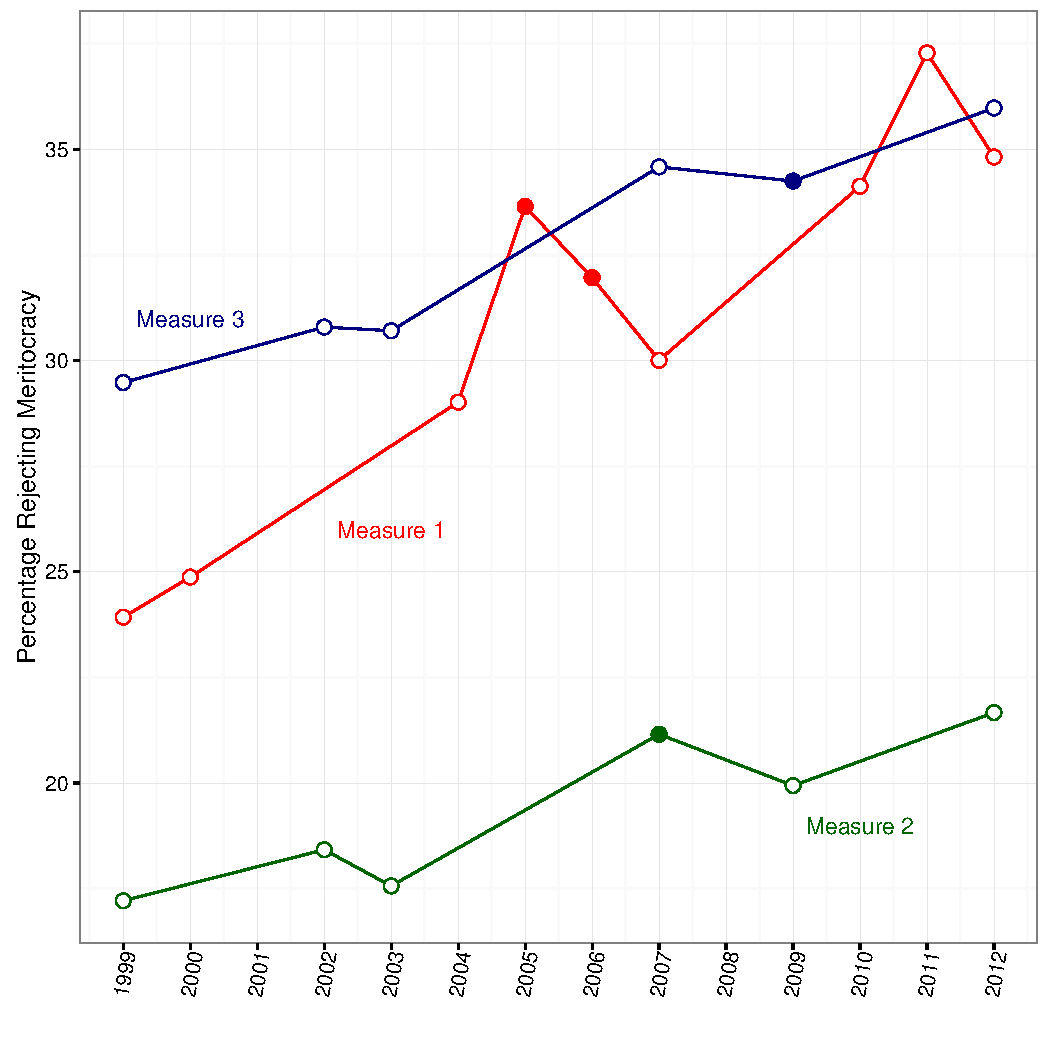
\includegraphics[width=5.25in]{../figures/04_three_measures_dv.pdf}
  \floatfoot{\emph{Notes}: The analyses presented in Table 1 of \citet[333]{Newman2015} were conducted on pooled observations with the dependent variable, rejection of meritocracy, measured in one of three different ways \citep[see][331]{Newman2015}.  Here, solid circles represent the data used by \citet{Newman2015}; hollow circles represent data in other available Pew surveys.  Plotting the percentage of (weighted) respondents to reject meritocracy by each of these measures reveals that the second measure results in much lower levels of rejection of meritocracy than either of the others and the third often yields considerably higher levels than the first.  In light of the evident lack of comparability of these three measures, pooling them into a single analysis cannot be justified.}
\end{figure}

